\documentclass[11pt,a4paper]{article}
\usepackage{fontspec}
\setmainfont{DejaVu Sans}[Scale=0.90]
\usepackage{amsmath,amssymb}
\usepackage[margin=2.2cm]{geometry}
\usepackage{booktabs,array,tabularx}
\usepackage{enumitem}
\usepackage{titlesec}
\usepackage{parskip}
\usepackage{graphicx}
\titlelabel{\thetitle.\quad}
\titleformat{\section}{\normalfont\large\bfseries}{\thesection.}{0.6em}{}
\titleformat{\subsection}{\normalfont\normalsize\bfseries}{\thesubsection}{0.6em}{}
\titlespacing*{\section}{0pt}{15pt}{5pt}
\titlespacing*{\subsection}{0pt}{11pt}{4pt}
\setlist[itemize]{leftmargin=1.4em,itemsep=1pt,topsep=3pt}
% Preserve fonts/margins; permit a final line-breaking pass for long prose.
\setlength{\emergencystretch}{2em}
\begin{document}
\begin{center}
{\Large\bfseries Analyse expérimentale : préparation FDTR}\\[4pt]
{\normalsize Faisceaux finis, transducteur, interfaces et paramètres de nuisance}\\[2pt]
{\small 16 septembre 2026 --- étude synthétique reproductible}
\end{center}

\section{Statut et objectif}
Aucune mesure de laboratoire ni géométrie confirmée n'a été fournie.
Cette note prépare l'expérience : modèle direct Fourier axisymétrique,
analyse locale des incertitudes, ajustement synthétique et liste des données
nécessaires. Elle ne fournit pas une conductivité mesurée ni une validation
du transport hydrodynamique dans l'AlN.

Le modèle 1D précédent reste utile pour les limites et les invariances.
Il ne suffit pas automatiquement à traiter un faisceau fini sur un métal.
La première question expérimentale est de savoir quels paramètres et quelles
corrections instrumentales peuvent être distingués dans la bande réellement mesurée.

\section{Modèle Fourier du signal mesuré}
Le cadre multicouche avec chauffage et détection gaussiens est classique :
D. G. Cahill, Rev. Sci. Instrum. \textbf{75}, 5119--5122 (2004),
doi:\allowbreak 10.1063/\allowbreak 1.1819431. Les conventions et la
normalisation employées ici sont dérivées explicitement ci-dessous.

Considérons des couches homogènes avec conductivités $\lambda_z,\lambda_r$,
capacité volumique $C$, épaisseur $d$ et résistance thermique surfacique $R$
à leur face inférieure. Le substrat est semi-infini.
À pulsation $p=i2\pi f$ et nombre d'onde radial $k$,
\[
 \gamma^2=\frac{\lambda_r k^2+Cp}{\lambda_z},\qquad
 Y=\lambda_z\gamma,\qquad Z_s=1/Y_s.
\]
Une couche au-dessus d'une impédance $Z_b$ a l'impédance
\[
 Z_t=\frac{Z_b+R+Y^{-1}\tanh(\gamma d)}
           {1+Y(Z_b+R)\tanh(\gamma d)}.
\]
La récurrence évite les matrices exponentiellement grandes.
Les interfaces sont parcourues dans leur ordre physique.
L'anisotropie admise est transverse, avec deux conductivités diagonales.

\subsection{Normalisation optique}
Les rayons $w_p,w_r$ sont ceux de l'intensité à $1/e^2$ :
\[
 q_{\rm pompe}(r)=\frac{2P_{\rm abs}}{\pi w_p^2}e^{-2r^2/w_p^2},
 \qquad W_{\rm sonde}(r)=\frac{2}{\pi w_r^2}e^{-2r^2/w_r^2}.
\]
Ainsi $\int q_{\rm pompe}\,dS=P_{\rm abs}$ et $\int W_{\rm sonde}\,dS=1$.
Avec $\eta=(w_p^2+w_r^2)/8$, la réponse en K/W est
\[
 H(f)=\frac{\overline T}{P_{\rm abs}}
 =\frac1{2\pi}\int_0^\infty k\,e^{-\eta k^2} Z_t(k,p)\,dk .
\]
On calcule l'intégrale complexe avant de prendre $\arg H$.
La phase moyenne locale n'est pas l'argument de la température moyenne.

Le changement $u=\sqrt\eta\,k$ donne une quadrature adaptative pondérée
par $u e^{-u^2}$. La limite supérieure numérique est $u=10$ ;
la queue gaussienne est négligeable pour les paramètres étudiés.
Le solveur vérifie le succès de la quadrature.
L'approximation 1D du \emph{même observable} est
$H_{\rm 1D}=2Z_t(0,p)/[\pi(w_p^2+w_r^2)]$.

\subsection{Limites et contrôles indépendants}
Pour un demi-espace isotrope sans couche,
\[
 H(f)=\frac{\operatorname{erfcx}(\sqrt{\eta p/a})}
 {4\lambda\sqrt{\pi\eta}}.
\]
Cette expression contrôle à la fois la normalisation de puissance, le
moyennage sonde et la limite DC. À faisceau très large, le résultat rejoint
$H_{\rm 1D}$. Une intégration indépendante en profondeur vérifie aussi
$T_z=-q/\lambda_z$ et $q_z=-(Cp+\lambda_rk^2)T$.

L'absorption est imposée à la surface. Ni pénétration optique dans le métal,
ni déséquilibre électron--phonon, ni conditions de bord GK 3D ne sont
implémentés ici. Ces effets doivent être évalués avant d'interpréter des données
qui les rendent importants. La note~15 explique pourquoi les interfaces
hydrodynamiques ne se réduisent pas automatiquement à un $R$ Fourier.

\section{Scénarios entièrement spécifiés}
Les valeurs ci-dessous sont des hypothèses de calcul, et non des propriétés
attribuées à l'échantillon réel. Les matériaux sont isotropes dans cette étude.
\begin{center}
\begin{tabular}{@{}lll@{}}
\toprule
Élément & Conductivité (W m$^{-1}$K$^{-1}$) & Autres valeurs\\
\midrule
Métal illustratif & 150 & $C=2{,}49\,10^6$, $d=80$ nm\\
Film illustratif & 60 ou 321 & $C=2{,}41\,10^6$, $d=500$ nm\\
Substrat & 35 & $C=3{,}03\,10^6$, semi-infini\\
Interface métal/film & --- & $R=10^{-8}$ m$^2$K/W\\
Interface film/substrat & --- & $R=2\,10^{-8}$ m$^2$K/W\\
Optique & --- & $w_p=10~\mu$m, $w_r=8~\mu$m\\
\bottomrule
\end{tabular}
\end{center}
Les capacités sont en J m$^{-3}$K$^{-1}$.
La valeur 321 n'est pas une mesure publiée pour un film de 500 nm :
elle sert ici uniquement de second scénario hypothétique.
On utilise 60 fréquences logarithmiques de 10 kHz à 200 MHz,
un écart-type de $0{,}01$ sur $\ln|H|$ et de $0{,}1^\circ$ sur la phase.
Les erreurs sont supposées gaussiennes, indépendantes et sans corrélation
entre fréquences ; cette hypothèse doit être contrôlée sur des répétitions.

\section{Calibration et information disponible}
Le signal instrumental est modélisé par
\[
 H_{\rm obs}(f)=\exp(g+i\phi_0-i2\pi f\,t_d)H(f).
\]
$g$ absorbe un gain d'amplitude inconnu, $\phi_0$ un décalage de phase,
$t_d$ un retard temporel. Les paramètres thermiques positifs sont
différenciés par rapport à leur logarithme. Le retard est exprimé en ns
et le décalage de phase en degrés dans le vecteur numérique.

Le vecteur complet contient dix paramètres : conductivité du film,
les deux résistances, les deux épaisseurs, la capacité du film,
un facteur commun sur les deux rayons, $g,\phi_0,t_d$.
La capacité du métal et les propriétés du substrat restent fixées.
L'incertitude publiée ci-dessous est donc encore conditionnelle à ces choix.

Pour des résidus blanchis $r$ et $J=\partial r/\partial x$,
la covariance locale est $(J^\top J+P)^{-1}$ lorsque le rang permet l'inversion.
La SVD des colonnes normalisées détecte les dépendances.
$P$ vaut zéro sans calibration indépendante.
Dans le scénario calibré, les écarts-types supposés sont :
$20\,\%$ sur $R_{\rm métal/film}$, $5\,\%$ sur l'épaisseur métallique,
$3\,\%$ sur celle du film, $5\,\%$ sur sa capacité, $3\,\%$ sur le facteur
de rayon, $0{,}02$ sur $g$, $0{,}1^\circ$ sur $\phi_0$ et $0{,}02$ ns
sur $t_d$. Pour les paramètres positifs, ce sont des écarts-types logarithmiques.
Ces informations sont hypothétiques ; elles ne sont pas fabriquées par les
données FDTR. Des étalonnages corrélés exigeraient une matrice $P$ non diagonale.

\section{Résultats du calcul synthétique}
Les valeurs sont les écarts-types locaux de $\ln\lambda$, présentés en pour cent.
L'approximation d'une erreur relative est valable seulement pour les petites valeurs.
\begin{center}
\begin{tabular}{@{}lrr@{}}
\toprule
Paramètres/information & $\lambda=60$ & $\lambda=321$\\
\midrule
$\lambda,R_{\rm film/substrat}$ seuls, amplitude + phase & 0,58 & 0,38\\
Les mêmes, phase seule & 0,67 & 0,43\\
Dix paramètres libres, amplitude + phase & 7,33 & 124,92\\
Dix paramètres + calibrations indépendantes & 6,16 & 4,03\\
Dix paramètres + calibrations, phase seule & 7,47 & 5,19\\
\bottomrule
\end{tabular}
\end{center}
La valeur 124,92\,\% signifie une information locale très faible ;
elle ne doit pas être présentée comme un intervalle gaussien fiable sur $\lambda$.
Une analyse de vraisemblance non linéaire serait nécessaire pour de vraies données.
Le simple succès d'un ajustement ne suffit pas non plus à établir une unicité globale.

L'erreur maximale de phase du modèle 1D atteint $30{,}91^\circ$ et
$31{,}65^\circ$ sur cette bande. Elle est due surtout à l'étalement radial
à basse fréquence. Il faut comparer l'erreur au bruit \emph{à chaque fréquence},
pas attribuer ce maximum à tout le spectre.
Les vecteurs complets sont conservés dans le fichier de résultats.

Un jeu synthétique, graine 20260916, avec $\lambda=60$ et les calibrations
centrées sur leurs vraies valeurs, donne
$\widehat\lambda=59{,}27$ W m$^{-1}$K$^{-1}$.
La somme des carrés des 120 résidus de données blanchis vaut $116{,}26$.
Trois initialisations rejoignent le même objectif pénalisé (environ $116{,}38$).
Ce contrôle valide le fonctionnement de l'estimateur dans le modèle choisi ;
il ne constitue ni une mesure d'AlN ni un test d'adéquation expérimentale.

\begin{center}
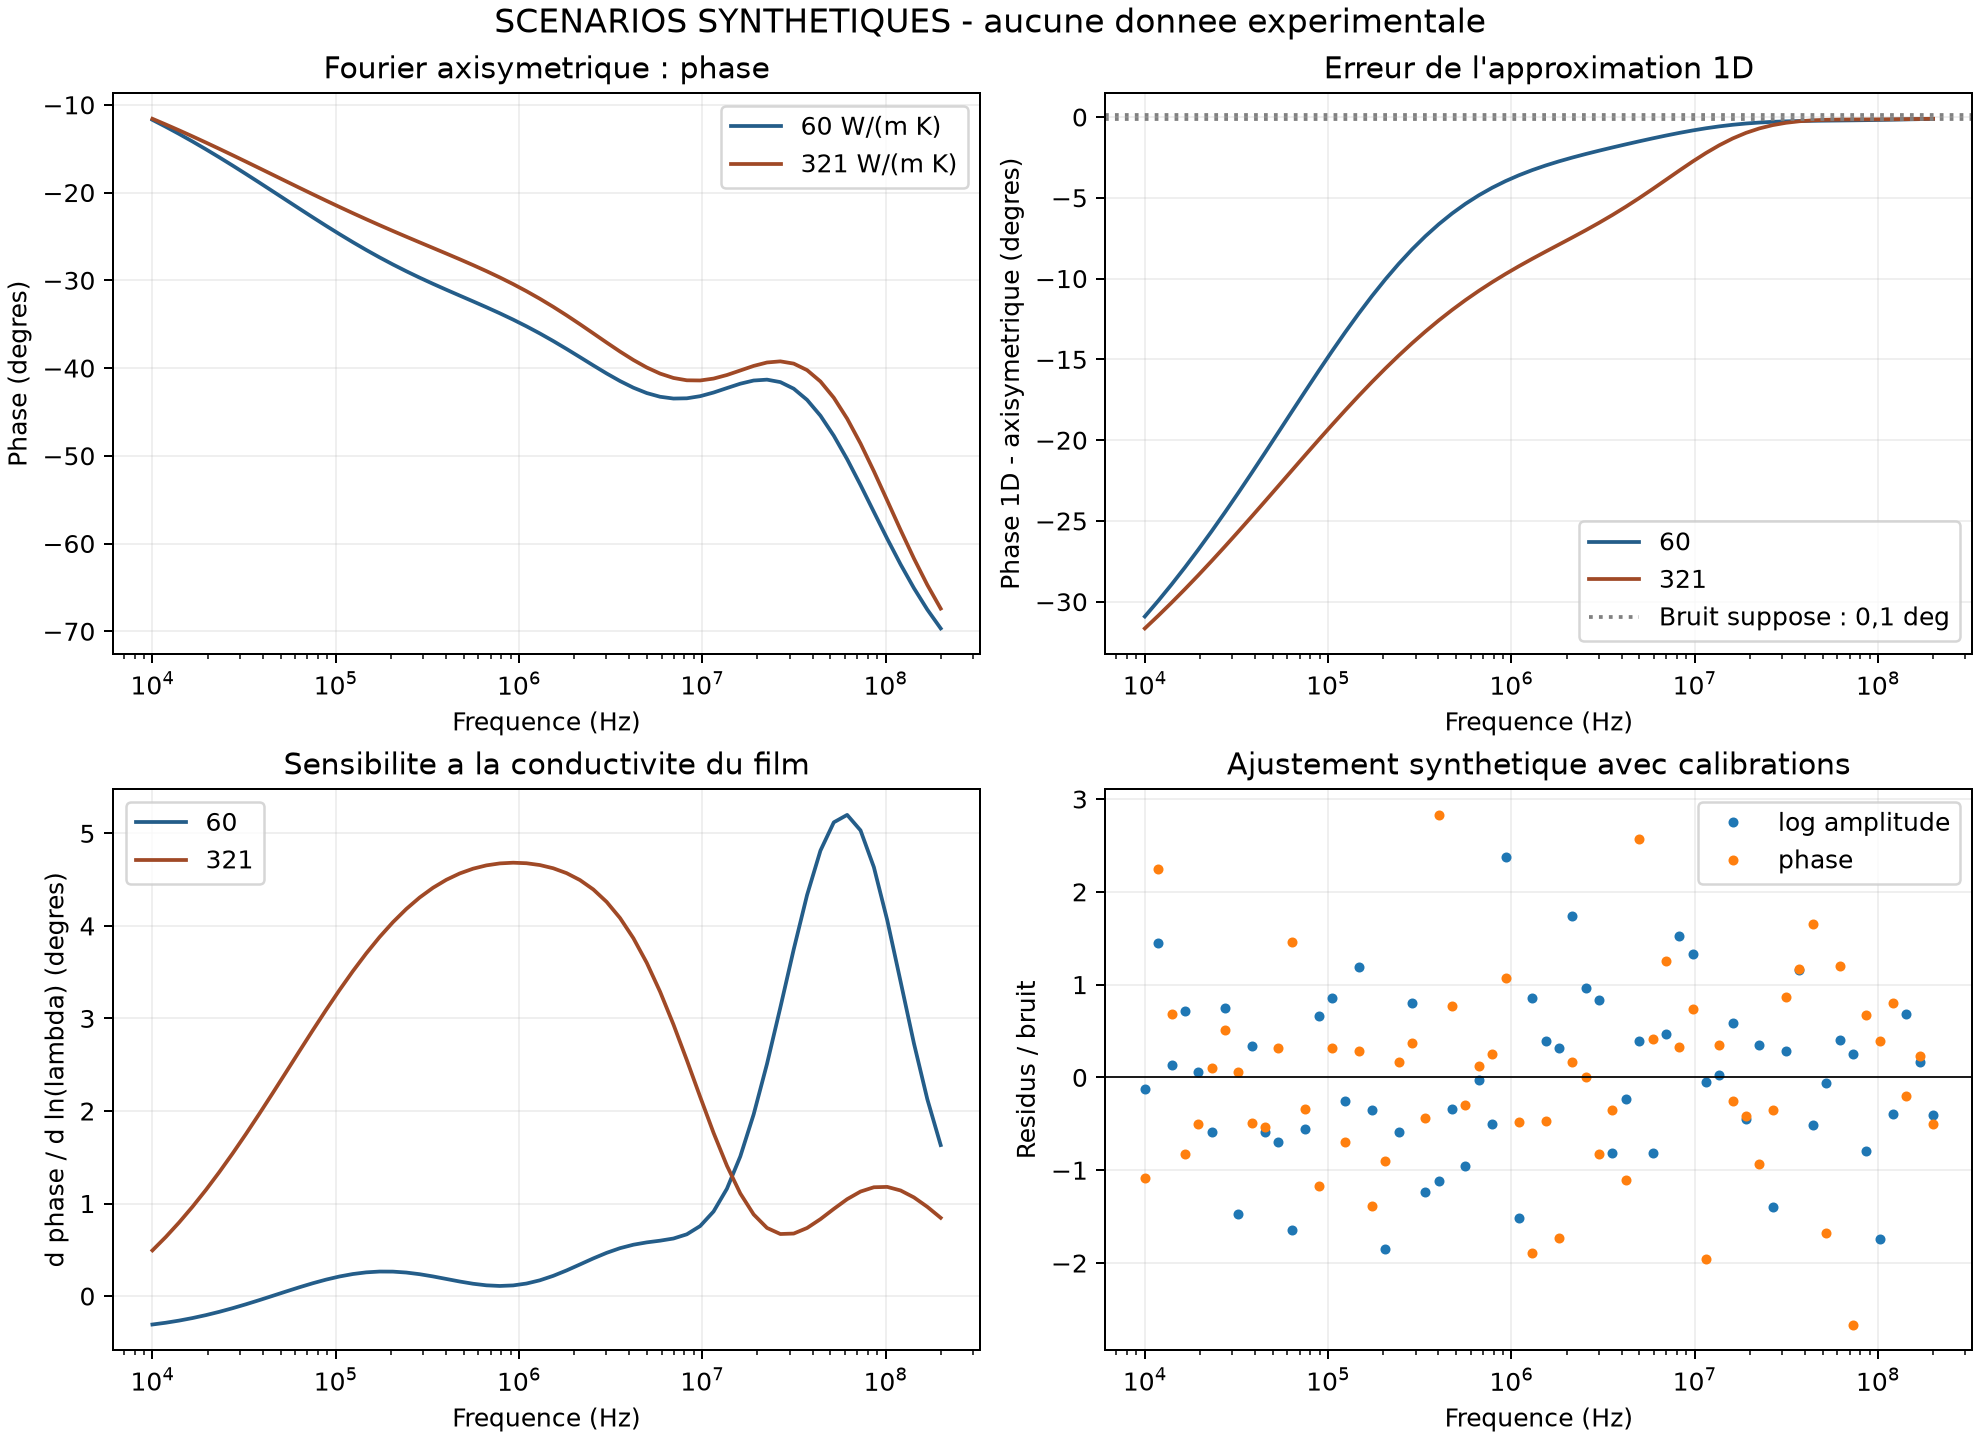
\includegraphics[width=\textwidth]{../figures/06_experimental_design.png}
\end{center}

\section{Protocole pour les données réelles}
\begin{enumerate}
\item Mesurer l'épaisseur et la composition du film, le transducteur et
les couches d'adhésion. Consigner orientation cristalline, substrat, température,
méthode de mesure et incertitude ; ne pas remplacer une valeur manquante
par le scénario illustratif sans le signaler.
\item Mesurer les deux rayons avec la convention $1/e^2$ et le décentrage.
Contrôler la dépendance à la puissance afin de rester dans la réponse linéaire.
Documenter puissance absorbée ou gain inconnu et coefficient de thermoréflectance.
\item Acquérir répétitions, référence de phase et étalonnage du retard.
Conserver les signaux complexes ou amplitude/phase avec leur convention,
et estimer le bruit en fonction de la fréquence, y compris ses corrélations.
\item Ajuster Fourier axisymétrique sur amplitude et phase avec paramètres
de nuisance explicites. Contrôler les résidus, plusieurs points de départ,
la stabilité au retrait d'une sous-bande et aux priors. Propager les
incertitudes des paramètres fixés si elles ne sont pas négligeables.
\item Tester séparément erreurs de rayon, épaisseur, interface et absorption
avant d'ajouter un temps de relaxation. Un gain d'ajustement doit être
comparé à la flexibilité supplémentaire et aux erreurs systématiques.
\item Pour revendiquer un temps non-Fourier, utiliser un modèle incluant
les conditions de bord et la géométrie appropriées ; comparer la vraisemblance
profilée avec le modèle Fourier. À $\tau=0$, le paramètre est sur une frontière :
un test de Wald standard ne suffit pas. Des simulations sous l'hypothèse
Fourier peuvent calibrer un test de rapport de vraisemblance.
\item Reproduire l'analyse sur un second rayon ou une seconde épaisseur,
si disponibles. L'objectif est une prédiction cohérente entre configurations,
pas seulement un ajustement unique.
\end{enumerate}

\section{Fichiers et limites restantes}
\texttt{src/fdtr.py} contient le modèle Fourier ;
\texttt{scripts/\allowbreak analyse\_\allowbreak experiment.py} produit
\texttt{theory/\allowbreak experimental\_\allowbreak results.json} et la figure~06.
Le modèle d'informations à recueillir est
\texttt{theory/\allowbreak experimental\_\allowbreak inputs.\allowbreak template.json}.
Lancer le script ne lit aucune donnée de laboratoire et ne transforme pas
ce modèle d'informations en fichier de mesures.

La dérivation grise est terminée et testée ; la correspondance avec les sources
accessibles est documentée. Restent les sources intégrales indisponibles,
le spectre propre à l'AlN, et la validation de l'échantillon et du banc.
Aucun ajustement expérimental n'est revendiqué avant réception de ces données.
\end{document}
